\documentclass[]{article}
\usepackage{lmodern}
\usepackage{amssymb,amsmath}
\usepackage{ifxetex,ifluatex}
\usepackage{fixltx2e} % provides \textsubscript
\ifnum 0\ifxetex 1\fi\ifluatex 1\fi=0 % if pdftex
  \usepackage[T1]{fontenc}
  \usepackage[utf8]{inputenc}
\else % if luatex or xelatex
  \ifxetex
    \usepackage{mathspec}
  \else
    \usepackage{fontspec}
  \fi
  \defaultfontfeatures{Ligatures=TeX,Scale=MatchLowercase}
\fi
% use upquote if available, for straight quotes in verbatim environments
\IfFileExists{upquote.sty}{\usepackage{upquote}}{}
% use microtype if available
\IfFileExists{microtype.sty}{%
\usepackage[]{microtype}
\UseMicrotypeSet[protrusion]{basicmath} % disable protrusion for tt fonts
}{}
\PassOptionsToPackage{hyphens}{url} % url is loaded by hyperref
\usepackage[unicode=true]{hyperref}
\hypersetup{
            pdftitle={In class},
            pdfauthor={Hyun Suk (Max) Ryoo (hr2ee)},
            pdfborder={0 0 0},
            breaklinks=true}
\urlstyle{same}  % don't use monospace font for urls
\usepackage[margin=1in]{geometry}
\usepackage{color}
\usepackage{fancyvrb}
\newcommand{\VerbBar}{|}
\newcommand{\VERB}{\Verb[commandchars=\\\{\}]}
\DefineVerbatimEnvironment{Highlighting}{Verbatim}{commandchars=\\\{\}}
% Add ',fontsize=\small' for more characters per line
\usepackage{framed}
\definecolor{shadecolor}{RGB}{248,248,248}
\newenvironment{Shaded}{\begin{snugshade}}{\end{snugshade}}
\newcommand{\KeywordTok}[1]{\textcolor[rgb]{0.13,0.29,0.53}{\textbf{#1}}}
\newcommand{\DataTypeTok}[1]{\textcolor[rgb]{0.13,0.29,0.53}{#1}}
\newcommand{\DecValTok}[1]{\textcolor[rgb]{0.00,0.00,0.81}{#1}}
\newcommand{\BaseNTok}[1]{\textcolor[rgb]{0.00,0.00,0.81}{#1}}
\newcommand{\FloatTok}[1]{\textcolor[rgb]{0.00,0.00,0.81}{#1}}
\newcommand{\ConstantTok}[1]{\textcolor[rgb]{0.00,0.00,0.00}{#1}}
\newcommand{\CharTok}[1]{\textcolor[rgb]{0.31,0.60,0.02}{#1}}
\newcommand{\SpecialCharTok}[1]{\textcolor[rgb]{0.00,0.00,0.00}{#1}}
\newcommand{\StringTok}[1]{\textcolor[rgb]{0.31,0.60,0.02}{#1}}
\newcommand{\VerbatimStringTok}[1]{\textcolor[rgb]{0.31,0.60,0.02}{#1}}
\newcommand{\SpecialStringTok}[1]{\textcolor[rgb]{0.31,0.60,0.02}{#1}}
\newcommand{\ImportTok}[1]{#1}
\newcommand{\CommentTok}[1]{\textcolor[rgb]{0.56,0.35,0.01}{\textit{#1}}}
\newcommand{\DocumentationTok}[1]{\textcolor[rgb]{0.56,0.35,0.01}{\textbf{\textit{#1}}}}
\newcommand{\AnnotationTok}[1]{\textcolor[rgb]{0.56,0.35,0.01}{\textbf{\textit{#1}}}}
\newcommand{\CommentVarTok}[1]{\textcolor[rgb]{0.56,0.35,0.01}{\textbf{\textit{#1}}}}
\newcommand{\OtherTok}[1]{\textcolor[rgb]{0.56,0.35,0.01}{#1}}
\newcommand{\FunctionTok}[1]{\textcolor[rgb]{0.00,0.00,0.00}{#1}}
\newcommand{\VariableTok}[1]{\textcolor[rgb]{0.00,0.00,0.00}{#1}}
\newcommand{\ControlFlowTok}[1]{\textcolor[rgb]{0.13,0.29,0.53}{\textbf{#1}}}
\newcommand{\OperatorTok}[1]{\textcolor[rgb]{0.81,0.36,0.00}{\textbf{#1}}}
\newcommand{\BuiltInTok}[1]{#1}
\newcommand{\ExtensionTok}[1]{#1}
\newcommand{\PreprocessorTok}[1]{\textcolor[rgb]{0.56,0.35,0.01}{\textit{#1}}}
\newcommand{\AttributeTok}[1]{\textcolor[rgb]{0.77,0.63,0.00}{#1}}
\newcommand{\RegionMarkerTok}[1]{#1}
\newcommand{\InformationTok}[1]{\textcolor[rgb]{0.56,0.35,0.01}{\textbf{\textit{#1}}}}
\newcommand{\WarningTok}[1]{\textcolor[rgb]{0.56,0.35,0.01}{\textbf{\textit{#1}}}}
\newcommand{\AlertTok}[1]{\textcolor[rgb]{0.94,0.16,0.16}{#1}}
\newcommand{\ErrorTok}[1]{\textcolor[rgb]{0.64,0.00,0.00}{\textbf{#1}}}
\newcommand{\NormalTok}[1]{#1}
\usepackage{graphicx,grffile}
\makeatletter
\def\maxwidth{\ifdim\Gin@nat@width>\linewidth\linewidth\else\Gin@nat@width\fi}
\def\maxheight{\ifdim\Gin@nat@height>\textheight\textheight\else\Gin@nat@height\fi}
\makeatother
% Scale images if necessary, so that they will not overflow the page
% margins by default, and it is still possible to overwrite the defaults
% using explicit options in \includegraphics[width, height, ...]{}
\setkeys{Gin}{width=\maxwidth,height=\maxheight,keepaspectratio}
\IfFileExists{parskip.sty}{%
\usepackage{parskip}
}{% else
\setlength{\parindent}{0pt}
\setlength{\parskip}{6pt plus 2pt minus 1pt}
}
\setlength{\emergencystretch}{3em}  % prevent overfull lines
\providecommand{\tightlist}{%
  \setlength{\itemsep}{0pt}\setlength{\parskip}{0pt}}
\setcounter{secnumdepth}{0}
% Redefines (sub)paragraphs to behave more like sections
\ifx\paragraph\undefined\else
\let\oldparagraph\paragraph
\renewcommand{\paragraph}[1]{\oldparagraph{#1}\mbox{}}
\fi
\ifx\subparagraph\undefined\else
\let\oldsubparagraph\subparagraph
\renewcommand{\subparagraph}[1]{\oldsubparagraph{#1}\mbox{}}
\fi

% set default figure placement to htbp
\makeatletter
\def\fps@figure{htbp}
\makeatother


\title{In class}
\author{Hyun Suk (Max) Ryoo (hr2ee)}
\date{9/28/2021}

\begin{document}
\maketitle

\begin{Shaded}
\begin{Highlighting}[]
\KeywordTok{library}\NormalTok{(tidyverse)}
\end{Highlighting}
\end{Shaded}

\begin{verbatim}
## Warning: package 'tidyverse' was built under R version 4.0.2
\end{verbatim}

\begin{verbatim}
## -- Attaching packages ----------------------------------------------------------------------------------------------------------------------- tidyverse 1.3.0 --
\end{verbatim}

\begin{verbatim}
## v ggplot2 3.3.2     v purrr   0.3.4
## v tibble  3.0.1     v dplyr   1.0.2
## v tidyr   1.1.2     v stringr 1.4.0
## v readr   1.4.0     v forcats 0.5.0
\end{verbatim}

\begin{verbatim}
## Warning: package 'ggplot2' was built under R version 4.0.2
\end{verbatim}

\begin{verbatim}
## Warning: package 'tidyr' was built under R version 4.0.2
\end{verbatim}

\begin{verbatim}
## Warning: package 'readr' was built under R version 4.0.2
\end{verbatim}

\begin{verbatim}
## Warning: package 'dplyr' was built under R version 4.0.2
\end{verbatim}

\begin{verbatim}
## Warning: package 'stringr' was built under R version 4.0.2
\end{verbatim}

\begin{verbatim}
## Warning: package 'forcats' was built under R version 4.0.2
\end{verbatim}

\begin{verbatim}
## -- Conflicts -------------------------------------------------------------------------------------------------------------------------- tidyverse_conflicts() --
## x dplyr::filter() masks stats::filter()
## x dplyr::lag()    masks stats::lag()
\end{verbatim}

\begin{Shaded}
\begin{Highlighting}[]
\KeywordTok{library}\NormalTok{(MASS)}
\end{Highlighting}
\end{Shaded}

\begin{verbatim}
## Warning: package 'MASS' was built under R version 4.0.2
\end{verbatim}

\begin{verbatim}
## 
## Attaching package: 'MASS'
\end{verbatim}

\begin{verbatim}
## The following object is masked from 'package:dplyr':
## 
##     select
\end{verbatim}

\section{1}\label{section}

Create a scatter plot of brain weight against body weight of land
mammals. Comment on the appearance of the plot. Do any assumptions for
simple linear regression appear to be violated? If so, which ones?

\begin{Shaded}
\begin{Highlighting}[]
\NormalTok{mammals }\OperatorTok
\StringTok{  }\KeywordTok{ggplot}\NormalTok{(}\KeywordTok{aes}\NormalTok{(body, brain)) }\OperatorTok{+}\StringTok{ }\KeywordTok{geom_point}\NormalTok{() }\OperatorTok{+}\StringTok{ }\KeywordTok{theme_bw}\NormalTok{()}
\end{Highlighting}
\end{Shaded}

\includegraphics{inclass_files/figure-latex/unnamed-chunk-2-1.pdf}

\subsection{Fit a simple linear regression to the data, and create the
corresponding residual
plot.}\label{fit-a-simple-linear-regression-to-the-data-and-create-the-corresponding-residual-plot.}

Do any assumptions for simple linear regression appear to be violated?
If so, which ones?

\begin{Shaded}
\begin{Highlighting}[]
\NormalTok{result <-}\StringTok{ }\KeywordTok{lm}\NormalTok{(brain}\OperatorTok{~}\NormalTok{body, }\DataTypeTok{data=}\NormalTok{mammals)}
\NormalTok{yhat =}\StringTok{ }\NormalTok{result}\OperatorTok{$}\NormalTok{fitted.values}
\NormalTok{res =}\StringTok{ }\NormalTok{result}\OperatorTok{$}\NormalTok{residuals}
\NormalTok{data =}\StringTok{ }\KeywordTok{data.frame}\NormalTok{(mammals, yhat, res)}
\NormalTok{data }\OperatorTok
\StringTok{  }\KeywordTok{ggplot}\NormalTok{(}\KeywordTok{aes}\NormalTok{(yhat, res)) }\OperatorTok{+}\StringTok{ }\KeywordTok{geom_point}\NormalTok{() }\OperatorTok{+}\StringTok{ }\KeywordTok{theme_bw}\NormalTok{() }\OperatorTok{+}\StringTok{ }\KeywordTok{geom_hline}\NormalTok{(}\DataTypeTok{yintercept=}\DecValTok{0}\NormalTok{, }\DataTypeTok{color=}\StringTok{"red"}\NormalTok{)}
\end{Highlighting}
\end{Shaded}

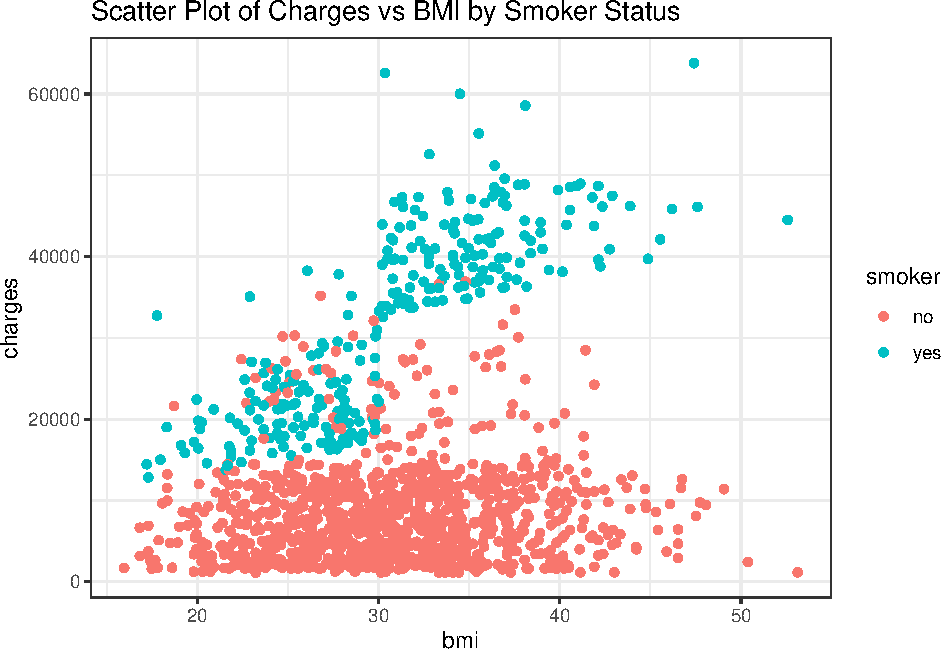
\includegraphics{inclass_files/figure-latex/unnamed-chunk-3-1.pdf}

\section{3}\label{section-1}

Based on your answers to parts 1 and 2, do we need to transform at least
one of the variables? Briefly explain.

\section{4}\label{section-2}

For the simple linear regression in part 2, create a Box Cox plot. What
transformation, if any, would you apply to the response variable?
Briefly explain. y = y\^{}0.1

\begin{Shaded}
\begin{Highlighting}[]
\NormalTok{result <-}\StringTok{ }\KeywordTok{lm}\NormalTok{(brain}\OperatorTok{~}\NormalTok{body, }\DataTypeTok{data=}\NormalTok{mammals)}
\KeywordTok{boxcox}\NormalTok{(result)}
\end{Highlighting}
\end{Shaded}

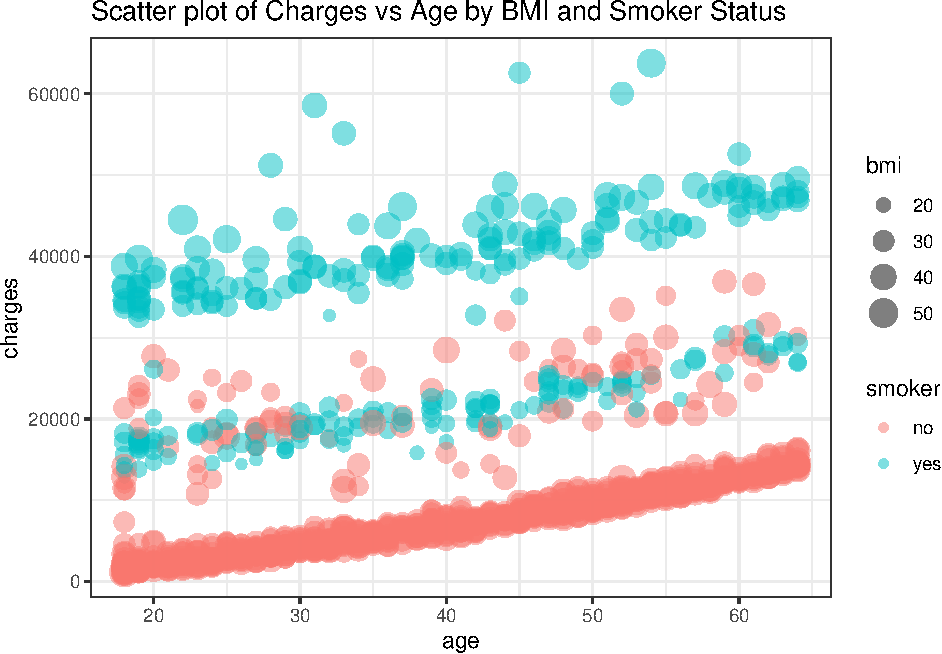
\includegraphics{inclass_files/figure-latex/unnamed-chunk-4-1.pdf}

\begin{Shaded}
\begin{Highlighting}[]
\KeywordTok{boxcox}\NormalTok{(result, }\DataTypeTok{lambda =} \KeywordTok{seq}\NormalTok{(}\OperatorTok{-}\FloatTok{0.05}\NormalTok{, }\FloatTok{0.2}\NormalTok{, }\DecValTok{1}\OperatorTok{/}\DecValTok{100}\NormalTok{))}
\end{Highlighting}
\end{Shaded}

\includegraphics{inclass_files/figure-latex/unnamed-chunk-4-2.pdf} \# 5
Apply the transformation you specified in part 4, and let y∗ denote the
transformed response variable. Create a scatterplot of y∗ against x.
Comment on the appearance of the plot. Do any assumptions for simple
linear regression appear to be violated? If so, which ones?

\begin{Shaded}
\begin{Highlighting}[]
\NormalTok{temp <-}\StringTok{ }\NormalTok{mammals}
\NormalTok{temp}\OperatorTok{$}\NormalTok{brain =}\StringTok{ }\NormalTok{temp}\OperatorTok{$}\NormalTok{brain}\OperatorTok{^}\FloatTok{0.075}
\NormalTok{temp }\OperatorTok
\StringTok{  }\KeywordTok{ggplot}\NormalTok{(}\KeywordTok{aes}\NormalTok{(body, brain)) }\OperatorTok{+}\StringTok{ }\KeywordTok{geom_point}\NormalTok{() }\OperatorTok{+}\StringTok{ }\KeywordTok{theme_bw}\NormalTok{()}
\end{Highlighting}
\end{Shaded}

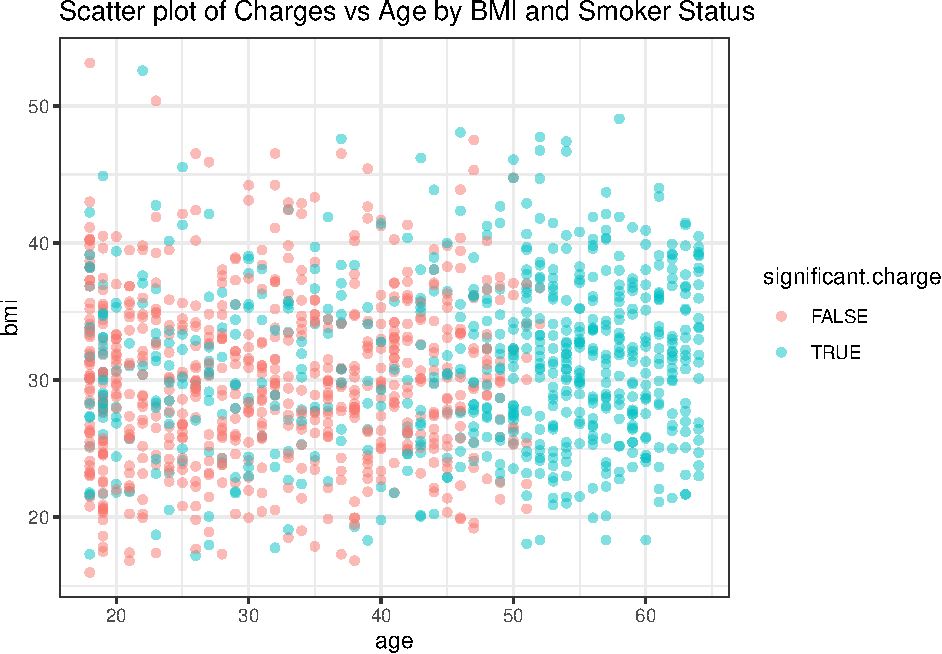
\includegraphics{inclass_files/figure-latex/unnamed-chunk-5-1.pdf}

\section{6}\label{section-3}

Fit a simple linear regression to y∗ against x, and create the
corresponding residual plot. Do any assumptions for simple linear
regression appear to be violated? If so, which ones?

\begin{Shaded}
\begin{Highlighting}[]
\NormalTok{result <-}\StringTok{ }\KeywordTok{lm}\NormalTok{(brain}\OperatorTok{~}\NormalTok{body, }\DataTypeTok{data=}\NormalTok{temp)}
\NormalTok{yhat =}\StringTok{ }\NormalTok{result}\OperatorTok{$}\NormalTok{fitted.values}
\NormalTok{res =}\StringTok{ }\NormalTok{result}\OperatorTok{$}\NormalTok{residuals}
\NormalTok{data =}\StringTok{ }\KeywordTok{data.frame}\NormalTok{(mammals, yhat, res)}
\NormalTok{data }\OperatorTok
\StringTok{  }\KeywordTok{ggplot}\NormalTok{(}\KeywordTok{aes}\NormalTok{(yhat, res)) }\OperatorTok{+}\StringTok{ }\KeywordTok{geom_point}\NormalTok{() }\OperatorTok{+}\StringTok{ }\KeywordTok{theme_bw}\NormalTok{() }\OperatorTok{+}\StringTok{ }\KeywordTok{geom_hline}\NormalTok{(}\DataTypeTok{yintercept=}\DecValTok{0}\NormalTok{, }\DataTypeTok{color=}\StringTok{"red"}\NormalTok{)}
\end{Highlighting}
\end{Shaded}

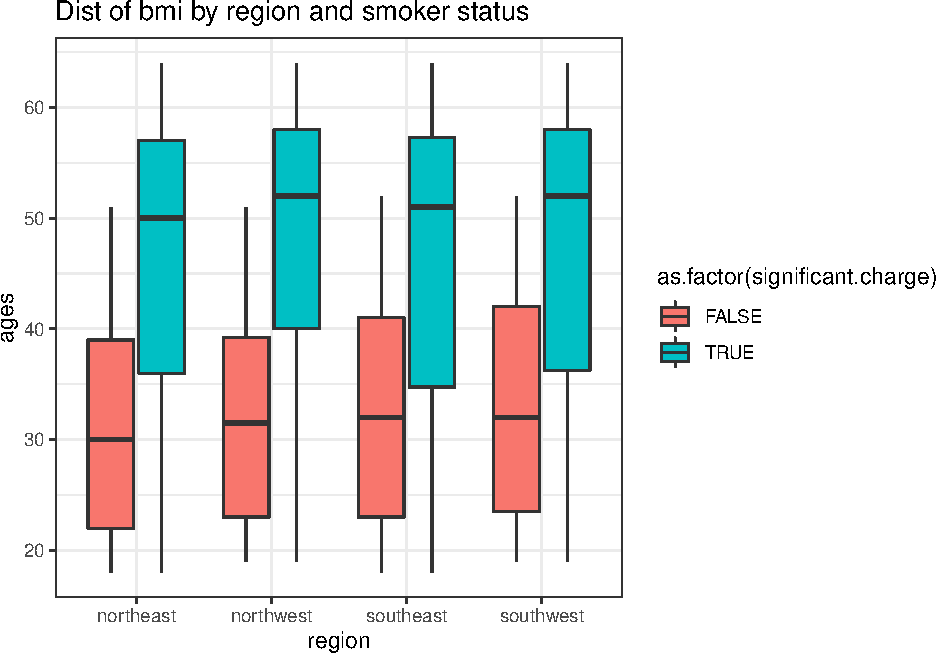
\includegraphics{inclass_files/figure-latex/unnamed-chunk-6-1.pdf}

\section{7}\label{section-4}

Do we need to transform the x variable? If yes, what transformation(s)
would you try? Briefly explain. Create a scatterplot of y∗ against x∗.
Do any assumptions for simple linear regression appear to be violated?
If so, which ones?

\begin{Shaded}
\begin{Highlighting}[]
\NormalTok{temp <-}\StringTok{ }\NormalTok{mammals}
\NormalTok{temp}\OperatorTok{$}\NormalTok{brain =}\StringTok{ }\NormalTok{temp}\OperatorTok{$}\NormalTok{brain}\OperatorTok{^}\FloatTok{0.075}
\NormalTok{temp }\OperatorTok
\StringTok{  }\KeywordTok{ggplot}\NormalTok{(}\KeywordTok{aes}\NormalTok{(}\KeywordTok{log}\NormalTok{(body), brain)) }\OperatorTok{+}\StringTok{ }\KeywordTok{geom_point}\NormalTok{() }\OperatorTok{+}\StringTok{ }\KeywordTok{theme_bw}\NormalTok{()}
\end{Highlighting}
\end{Shaded}

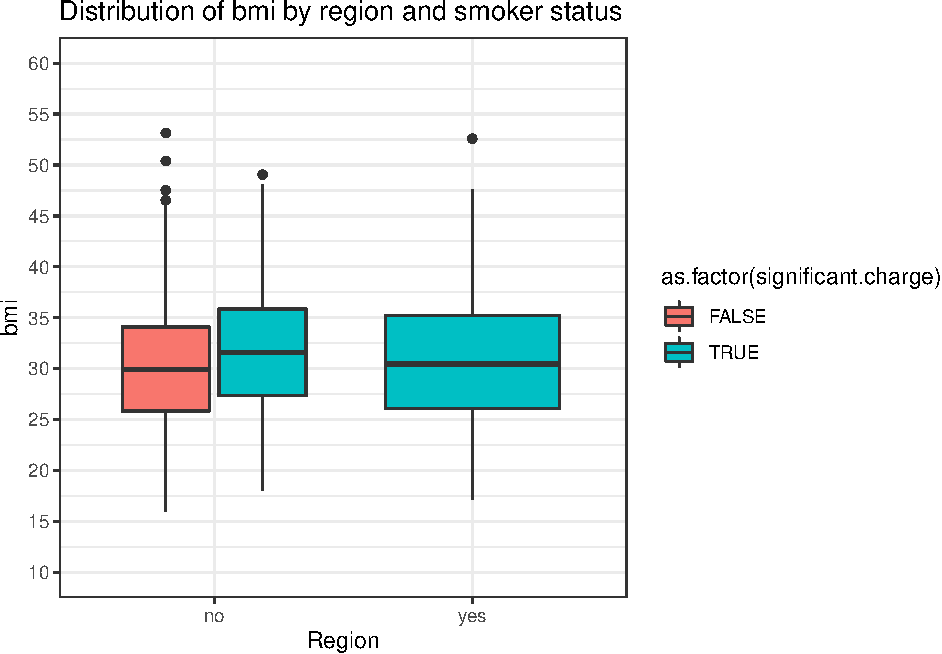
\includegraphics{inclass_files/figure-latex/unnamed-chunk-7-1.pdf}

\section{8}\label{section-5}

Fit a simple linear regression to y∗ against x∗, and create the
corresponding residual plot. Do any assumptions for simple linear
regression appear to be violated? If so, which ones? If the assumptions
are not met, repeat with a different transformation on the predictor
until you are satisfied.

\begin{Shaded}
\begin{Highlighting}[]
\NormalTok{result <-}\StringTok{ }\KeywordTok{lm}\NormalTok{(brain}\OperatorTok{~}\KeywordTok{log}\NormalTok{(body), }\DataTypeTok{data=}\NormalTok{temp)}
\NormalTok{yhat =}\StringTok{ }\NormalTok{result}\OperatorTok{$}\NormalTok{fitted.values}
\NormalTok{res =}\StringTok{ }\NormalTok{result}\OperatorTok{$}\NormalTok{residuals}
\NormalTok{data =}\StringTok{ }\KeywordTok{data.frame}\NormalTok{(mammals, yhat, res)}
\NormalTok{data }\OperatorTok
\StringTok{  }\KeywordTok{ggplot}\NormalTok{(}\KeywordTok{aes}\NormalTok{(yhat, res)) }\OperatorTok{+}\StringTok{ }\KeywordTok{geom_point}\NormalTok{() }\OperatorTok{+}\StringTok{ }\KeywordTok{theme_bw}\NormalTok{() }\OperatorTok{+}\StringTok{ }\KeywordTok{geom_hline}\NormalTok{(}\DataTypeTok{yintercept=}\DecValTok{0}\NormalTok{, }\DataTypeTok{color=}\StringTok{"red"}\NormalTok{)}
\end{Highlighting}
\end{Shaded}

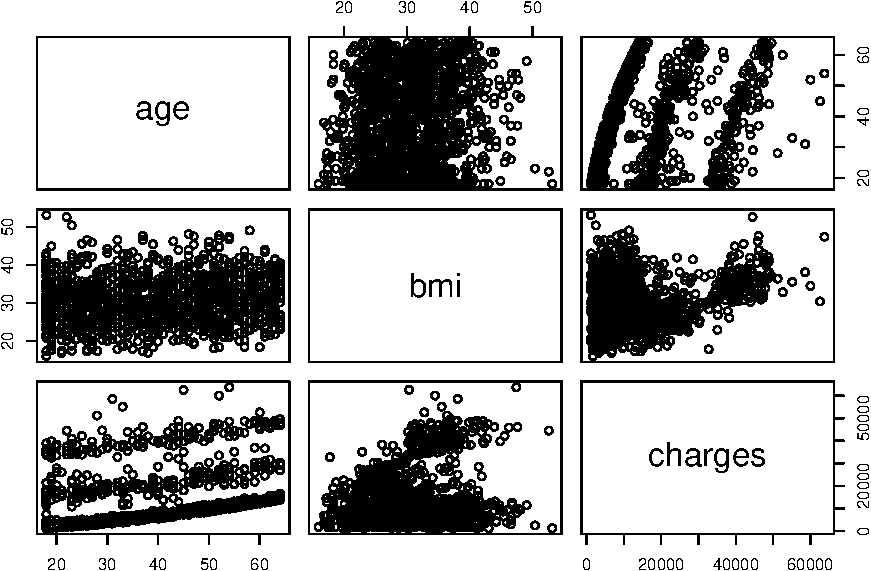
\includegraphics{inclass_files/figure-latex/unnamed-chunk-8-1.pdf}

\section{9}\label{section-6}

Create an ACF plot of the residuals. Comment if assumptions are met for
linear regression.

\begin{Shaded}
\begin{Highlighting}[]
\KeywordTok{acf}\NormalTok{(result}\OperatorTok{$}\NormalTok{residuals, }\DataTypeTok{main=}\StringTok{"ACF Plot of Residuals with ystar"}\NormalTok{)}
\end{Highlighting}
\end{Shaded}

\includegraphics{inclass_files/figure-latex/unnamed-chunk-9-1.pdf}

\section{10}\label{section-7}

Create a QQ plot of the residuals. Comment if assumptions are met for
linear regression.

\begin{Shaded}
\begin{Highlighting}[]
\KeywordTok{qqnorm}\NormalTok{(result}\OperatorTok{$}\NormalTok{residuals)}
\end{Highlighting}
\end{Shaded}

\includegraphics{inclass_files/figure-latex/unnamed-chunk-10-1.pdf}

\section{11}\label{section-8}

Write out the regression equation, and if possible, interpret the slope
of the regression.

\begin{Shaded}
\begin{Highlighting}[]
\NormalTok{result}
\end{Highlighting}
\end{Shaded}

\begin{verbatim}
## 
## Call:
## lm(formula = brain ~ log(body), data = temp)
## 
## Coefficients:
## (Intercept)    log(body)  
##     1.18940      0.07276
\end{verbatim}

\(y^{0.05} = 1.00008012 + 0.002822(log(x))\)

\end{document}
